\documentclass[12pt,a4paper]{article}

\usepackage[utf8]{inputenc}
\usepackage[T1]{fontenc}
\usepackage{polski}

\usepackage{amsthm}
\usepackage{amsmath}
\usepackage{amsfonts}
\usepackage{amssymb}
\usepackage{pgfplots}
\usepackage{tikz}
\usepackage{lmodern}	%fancy font
\usepackage{textcomp}

\usepackage{indentfirst}
\usepackage{graphicx}
\usepackage{caption}
\usepackage{subcaption}
\usepackage{siunitx}
\usepackage{here}


\setlength{\textheight}{24cm}
\setlength{\textwidth}{15.92cm}
\setlength{\footskip}{10mm}
\setlength{\oddsidemargin}{0mm}
\setlength{\evensidemargin}{0mm}
\setlength{\topmargin}{0mm}
\setlength{\headsep}{5mm}
\usepackage{tikz}
\usepackage{lmodern}	%fancy font
\usepackage{textcomp}

\usepackage{indentfirst}
\usepackage{graphicx}
\usepackage{caption}
\usepackage{subcaption}
\usepackage{siunitx}
\usepackage{here}
\usepackage[margin=1in]{geometry}% Just for this example
\setlength{\parindent}{0pt}% Just for this example
\setlength{\textheight}{24cm}
\setlength{\textwidth}{15.92cm}
\setlength{\footskip}{10mm}
\setlength{\oddsidemargin}{0mm}
\setlength{\evensidemargin}{0mm}
\setlength{\topmargin}{0mm}


\begin{document}

\begin{table}[H]
\label{my-label}
\begin{tabular}[width=\textwidth, height=0.5]{|c|c|}
\hline
									           					&                           \\

\includegraphics[height=3cm]{img/logo}             					& \textbf{Technika cyfrowa} \\ \hline
\multicolumn{1}{|l|}{\textbf{Temat ćwiczenia}} 					& \textbf{Numer ćwiczenia}  \\
\multicolumn{1}{|l|}{Minimalizacja i praktyczna realizacja złożonych funkcji logicznych}	& 2                         \\ \hline
\multicolumn{1}{|l|}{\textbf{Wykonawca}}       & \textbf{Ocena}            \\
\multicolumn{1}{|l|}{Łukasz Nawojowski}          &                           \\ \hline
\end{tabular}
\end{table}

\section{Cel ćwiczenia}
Zapoznanie się z różnymi rodzajami przerzutników i zbudowanie z nich rejestrów SISO, SIPO, PIPO i PISO.

\section{Przebieg ćwiczenia}
\subsection{Asynchroniczny przerzutnik RS}
\begin{figure}[H]
\centering
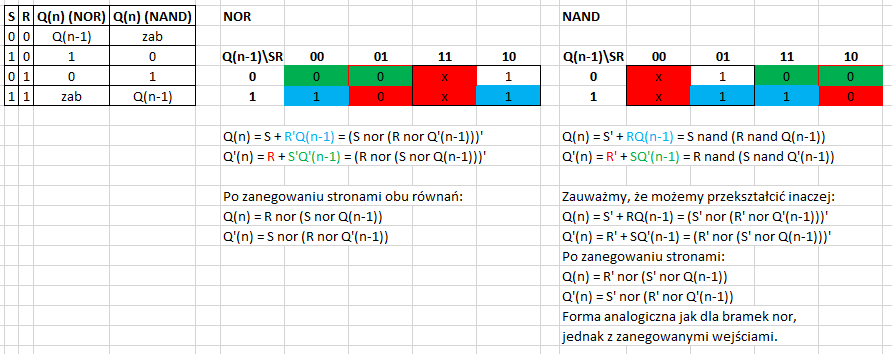
\includegraphics[width=\textwidth]{img/3a_karnaugh}
\end{figure}
\begin{figure}[H]
\centering
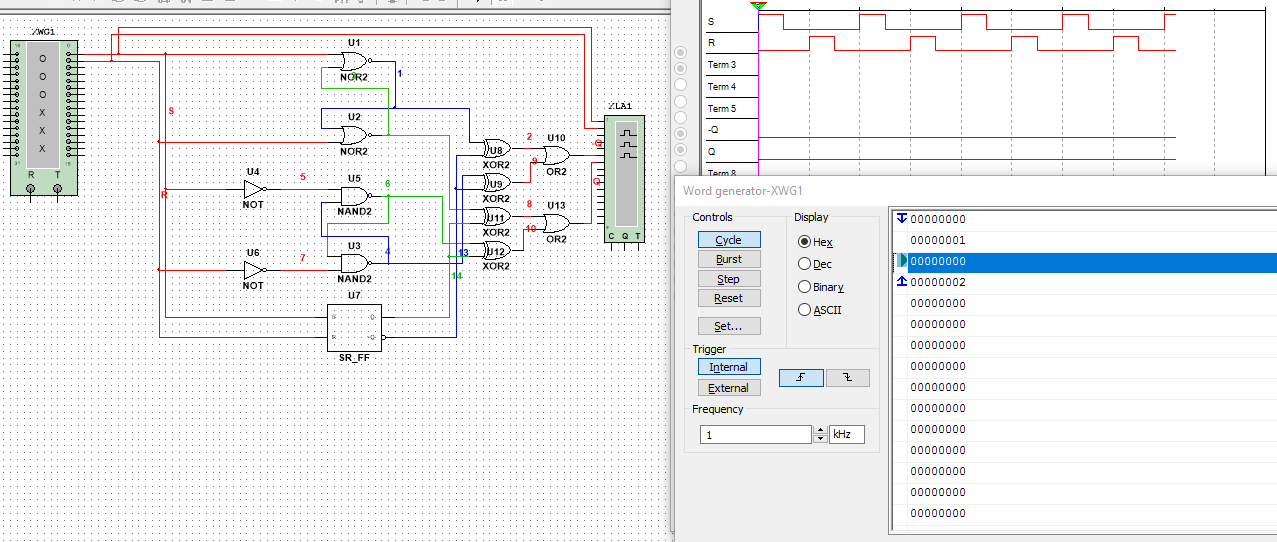
\includegraphics[width=\textwidth]{img/3a}
\end{figure}

Widzimy, że przerzutnik działa zgodnie z przewidywaniami. Przerzutnik oparty o bramki NAND działa tak, jakbyśmy zanegowali wejścia przerzutnika opartego o bramki NOR.

\subsection{Synchroniczny przerzutnik RS}
%\begin{figure}[H]
%\centering
%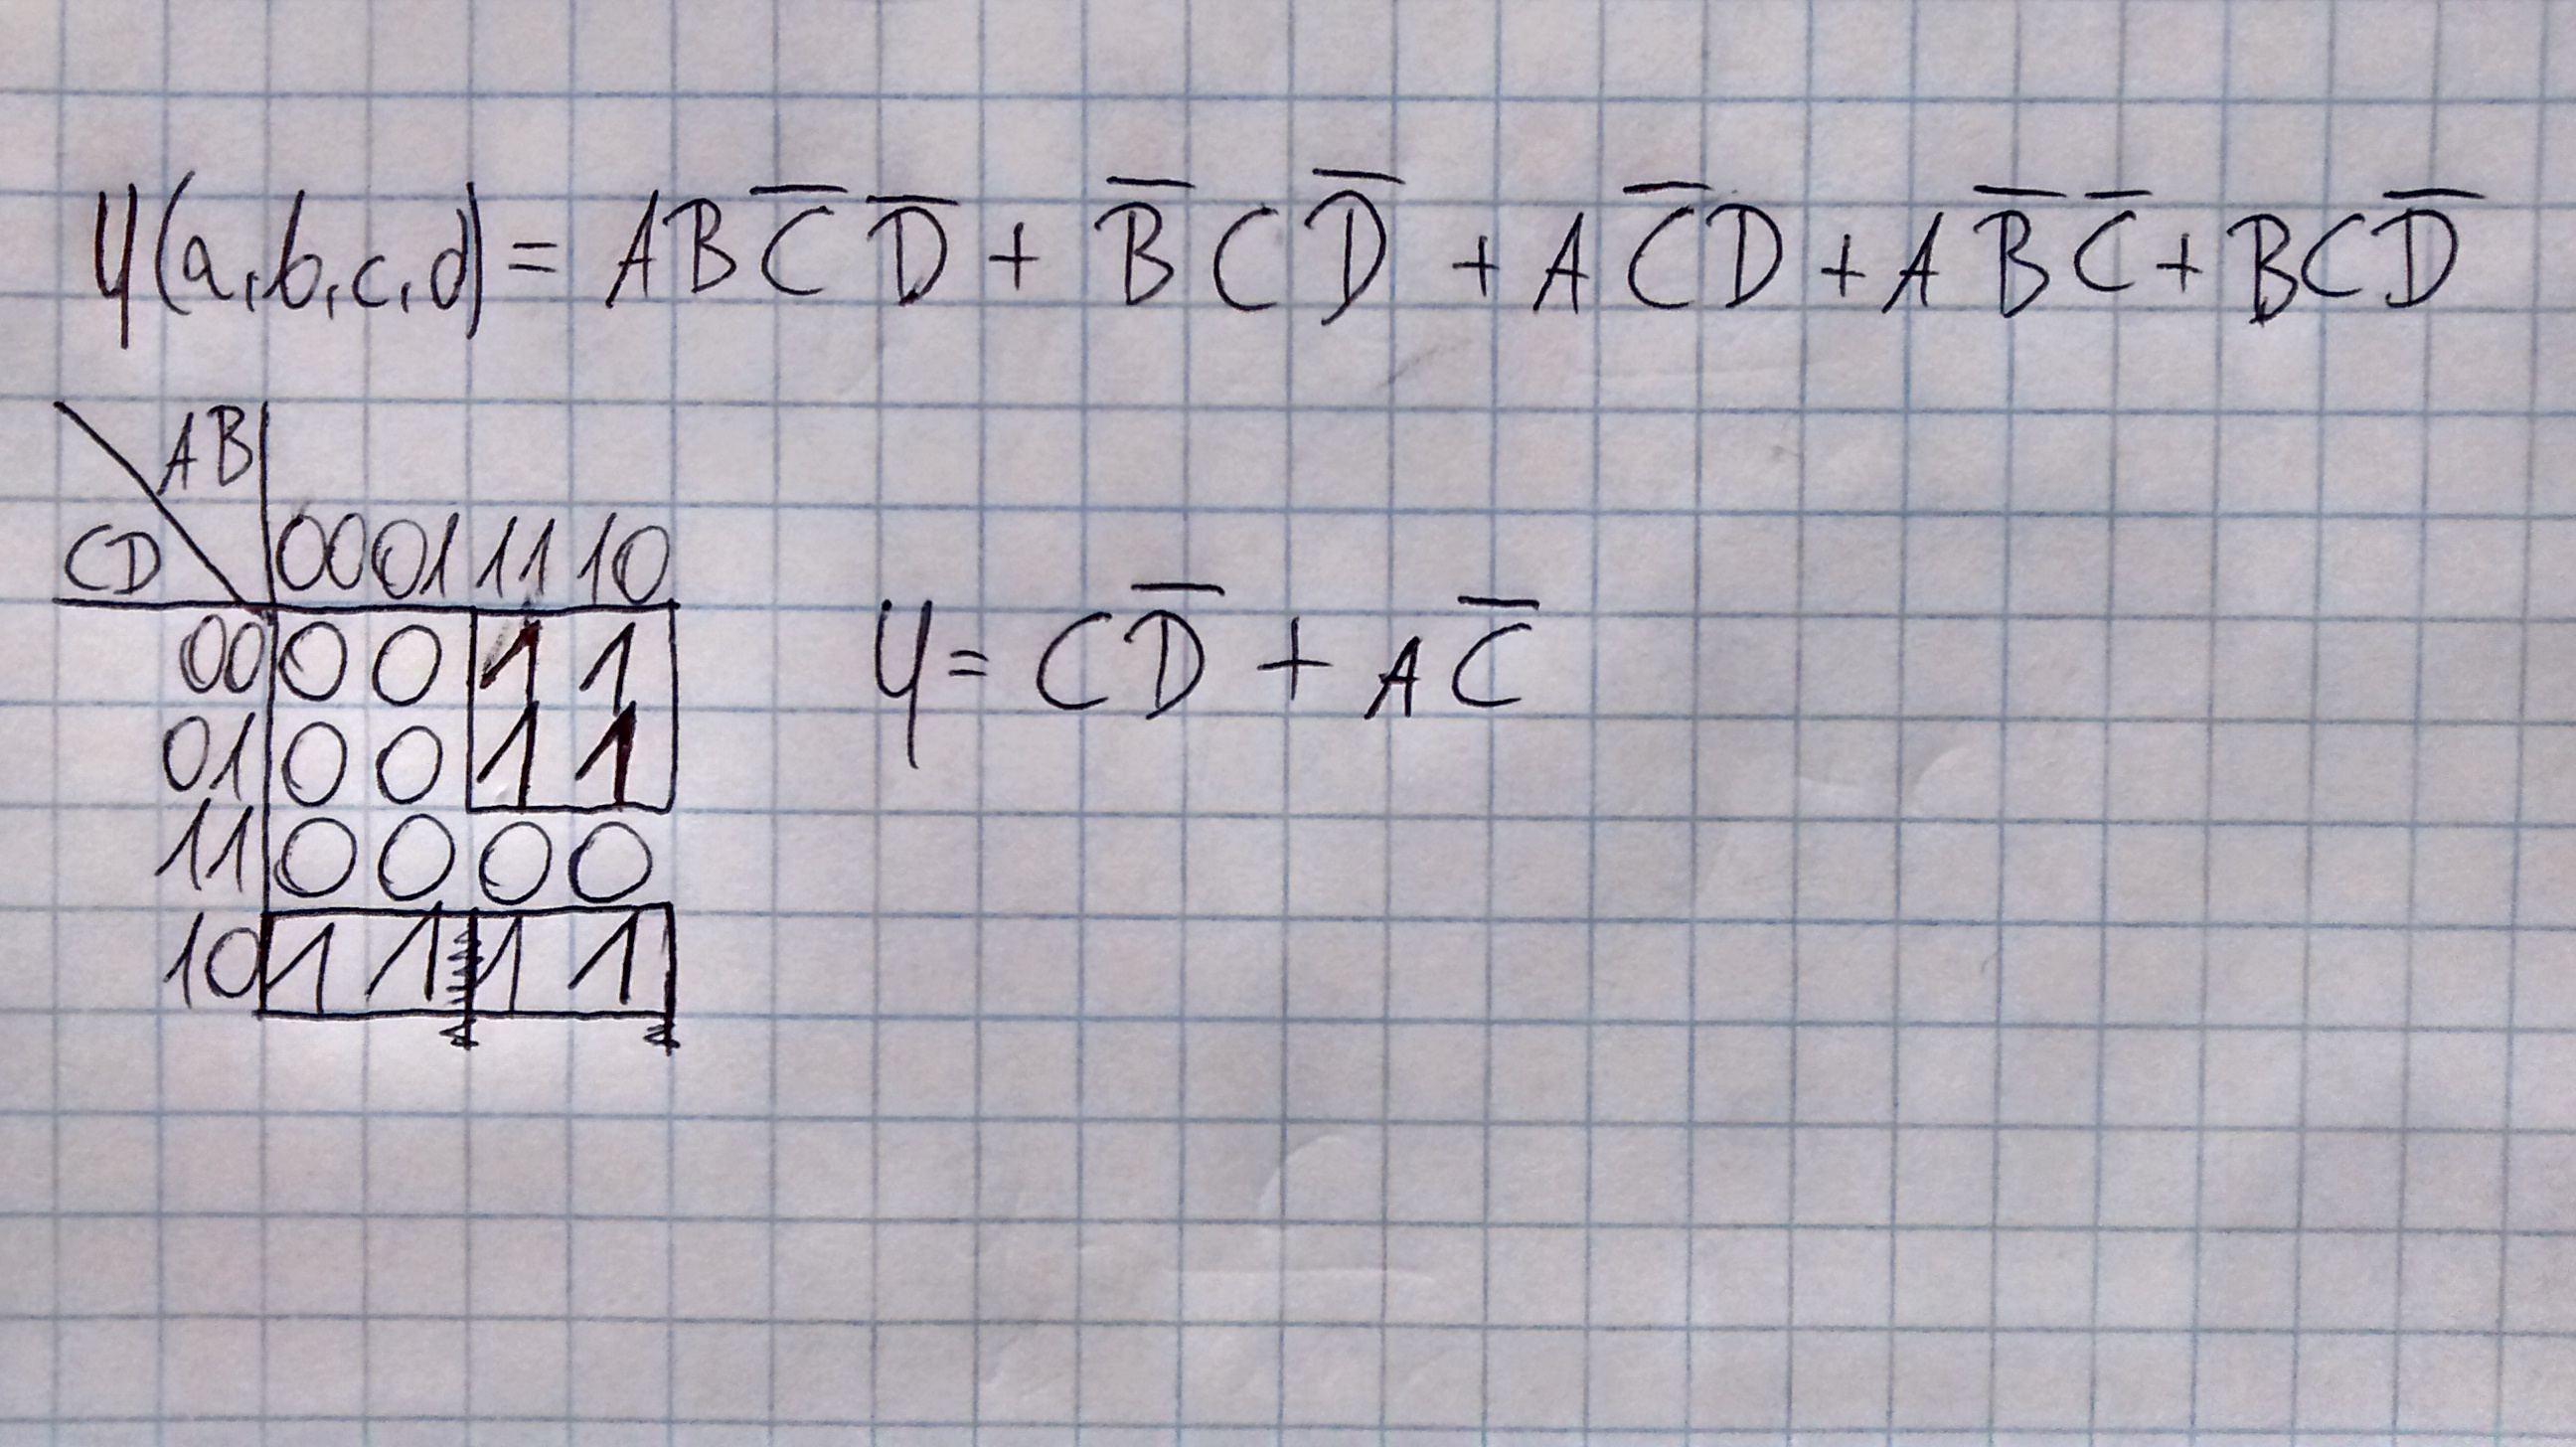
\includegraphics[width=\textwidth]{min_func_karnaugh}
%\end{figure}



\subsection{Synchroniczny przerzutnik JK}
%\begin{figure}[H]
%\centering
%\includegraphics[width=0.25\textwidth]{7seg/segconf}
%\end{figure}



\subsection{Przerzutnik D na podstawie asynchronicznego przerzutnika RS}
%\begin{figure}[H]
%\centering
%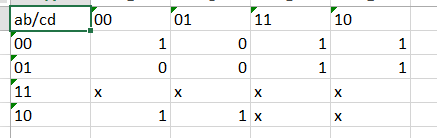
\includegraphics[width=0.3\textwidth]{7seg/seg0}
%\end{figure}

\subsection{Przerzutnik T na podstawie synchronicznego przerzutnika D}
%\begin{figure}[H]
%\centering
%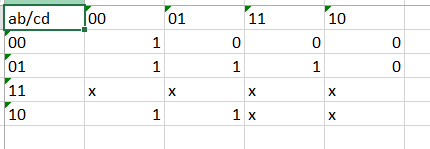
\includegraphics[width=0.3\textwidth]{7seg/seg1}
%\end{figure}

\subsection{Przerzutnik D na podstawie synchronicznego przerzutnika JK}
%\begin{figure}[H]
%\centering
%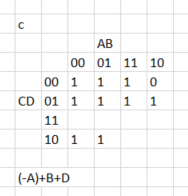
\includegraphics[width=0.3\textwidth]{7seg/seg2}
%\end{figure}

\subsection{Przerzutnik T na podstawie synchronicznego przerzutnika JK}
%\begin{figure}[H]
%\centering
%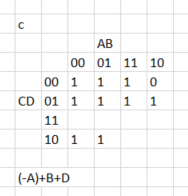
\includegraphics[width=0.3\textwidth]{7seg/seg2}
%\end{figure}

\subsection{Rejestry na podstawie synchronicznych przerzutników D}
\subsubsection{Rejestr SISO}
%\begin{figure}[H]
%\centering
%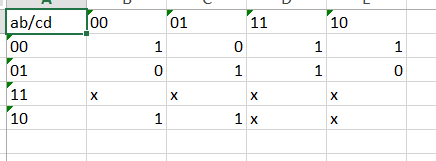
\includegraphics[width=0.3\textwidth]{7seg/seg6}
%\end{figure}

\subsubsection{Rejestr SIPO}
%\begin{figure}[H]
%\centering
%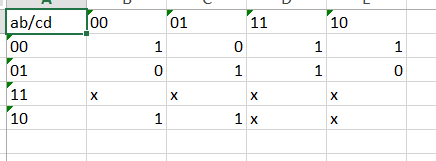
\includegraphics[width=0.3\textwidth]{7seg/seg6}
%\end{figure}

\subsubsection{Rejestr PIPO}
%\begin{figure}[H]
%\centering
%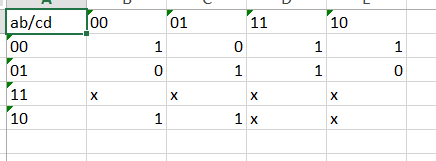
\includegraphics[width=0.3\textwidth]{7seg/seg6}
%\end{figure}

\subsubsection{Rejestr PISO}
%\begin{figure}[H]
%\centering
%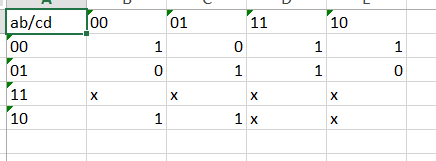
\includegraphics[width=0.3\textwidth]{7seg/seg6}
%\end{figure}

Widzimy jak przerzutniki mogą posłużyć ku wyjściu na kolejny poziom abstrakcji - do zbudowania rejestrów, skąd już tylko niewielki krok do asemblera i ciekawszych języków wysokiego poziomu.

\end{document}
